%!TEX root = slides.tex

\section[Session 1]{Session 1: Evolutionary genetics of associations among
genotypes, phenotypes, and environments}

\begin{frame}
\frametitle{Definitions}
\begin{block}{Local adaptation}
\centering
Individuals of a \textbf{local} population have higher relative fitness in 
their \textbf{local} environment compared to individuals from other 
environments.
\end{block}

\begin{block}{}
\begin{itemize}
\item{Patterns in each habitat are independent of each other}
\item{Affected by gene flow}
\item{Confounded by drift, temporal sampling}
\item{Process driven by divergent selection $\longleftrightarrow$ drift}
\end{itemize}
\end{block}
\tiny
\citet{Kawecki:2004hxa}
\end{frame}

\begin{frame}
\frametitle{Therefore, local adaptation is:}
\Large
\begin{block}{}
''...patterns and processes observed across local populations of the same
species connected, at least potentially, by dispersal and gene flow.''
\citep{Kawecki:2004hxa}.
\end{block}
\end{frame}

\begin{frame}
\frametitle{And any adaptation is:}
\Large
\begin{block}{}
a phenotype (or some aspect of) which increases Darwinian fitness over other 
forms of the phenotype.
\end{block}

\begin{block}{Question}
\centering
What is Darwinian fitness?
\end{block}
\end{frame}

\begin{frame}
\frametitle{Fitness}
\begin{block}{Absolute fitness}
\centering
\large
\begin{equation}
W_{abs} = \frac{N_{after}}{N_{before}}
\end{equation}
\end{block}

\begin{block}{Relative fitness}
\centering
$W_{A1,A1} = 0.75, W_{A1,A2} = 0.25, W_{A2,A2} = 0.95$

\vspace{2em}

$W_{A2,A2} = 1.0$\\ \vspace{1em}
$W_{A1,A1} = \frac{0.75}{0.95} = 0.79$\\ \vspace{1em}
$W_{A1,A2} = \frac{0.25}{0.95} = 0.26$\\ \vspace{1em}
\tiny
\end{block}
\end{frame}

\begin{frame}
\frametitle{Local adaptation review}
\begin{block}{Question}
\large
What happens to the genetic variance among populations in fitness-related
traits in the presence of gene flow but no selection?
\end{block}
\end{frame}

\begin{frame}
\frametitle{Local adaptation review}
\begin{block}{Questions}
\large
Given standing genetic variation in fitness-related traits in populations
connected by gene flow, what can you say about: 
\begin{enumerate}
\item{the presence/absence of natural selection acting in the populations?}
\item{the relationship between the trait and the environment?}
\end{enumerate}
\end{block}
\end{frame}

\begin{frame}
\frametitle{The genetic basis for local adaptation}
\begin{block}{Antagonistic pleiotropy vs conditional
neutrality}
\centering
\includegraphics[width=0.75\textwidth]{salvo_fig1}\\
\tiny
Adapted from \citet[Figure 1]{Savolainen:2013dfa}
\end{block}
\end{frame}

\begin{frame}
\frametitle{Local adaptation}
\begin{block}{In summary}
\begin{itemize}
\item{Local adaptation results from a balance between selection and gene flow
(migration)}
\item{Selection pressures can also vary spatially and temporally
(recolonization/extinction)}
\item{Phenotypic plasticity can also play a role in local adaptation}
\end{itemize}
\end{block}
\tiny
*Adapted from \citet{Savolainen:2013dfa}
\end{frame}

\begin{frame}
\frametitle{Local adaption}
\begin{block}{Questions}

\begin{itemize}
\item{What is the potential for a populations exhibiting highly plastic traits
to become locally adapated?}
\item{Can local adaptation occur when fitness only increases in each
environment?}
\end{itemize}
\end{block}
\end{frame}



\begin{frame}
\frametitle{Methods to detect local adaptation}
\begin{block}{Current approaches*}{}
\begin{itemize}
\item{QTL-mapping}
\item{Population genetics}
\item{Association mapping}
\end{itemize}
\end{block}
\tiny
*Adapted from \citet{Savolainen:2013dfa}
\end{frame}

\begin{frame}
\frametitle{LD and marker density}
\begin{block}{How much sequencing do you need?}
\centering
\includegraphics[width=0.7\textwidth]{ld_decay}
\end{block}
\end{frame}


\begin{frame}
\frametitle{Methods to detect local adaptation}
\begin{block}{QTL}
\begin{itemize}
\item{Can operate on a reduced set of markers (GBS: RAD, ddRAD)}
\item{Does not require a reference genome}
\item{Need a linkage map, large sample sizes, many crosses}
\end{itemize}
\end{block}
\end{frame}

\begin{frame}
\frametitle{QTL in \textit{Boechera stricta}}
\begin{columns}

\begin{column}{0.4\textwidth}
\footnotesize
\begin{block}{Flowering time}
\begin{itemize}
\item{Supports local adaptation due to favored native alleles at 
both sites($\bar{\Delta} f_C = 0.016, \bar{\Delta} f_M = 
0.048, p < 0.001$)}
\item{2.8\% of genome is AP, 8.1\% CN}
\item{$\sim$all AP linked to \textit{nFT}}
\end{itemize}
\end{block}


\end{column}

\begin{column}{0.6\textwidth}
\centering
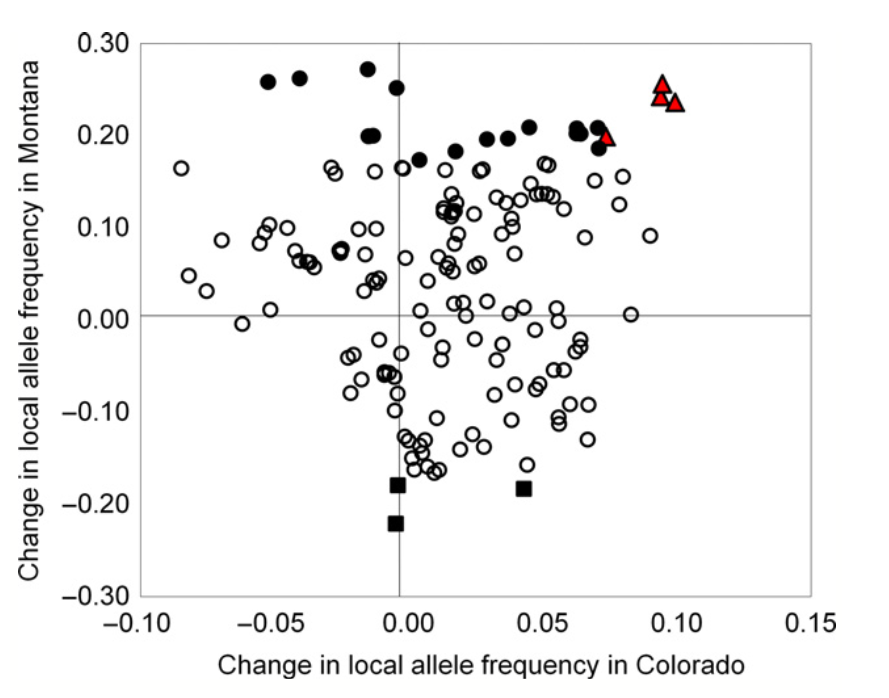
\includegraphics[width=0.9\textwidth]{boechera.png}\\
\tiny
Adapted from \citet[Figure 1]{Anderson:2012cb}

\end{column}

	
\end{columns}

\end{frame}

\begin{frame}
\frametitle{QTL in \textit{Boechera stricta}}
\begin{block}{\textit{nFT QTL $\times$ E}}
\centering
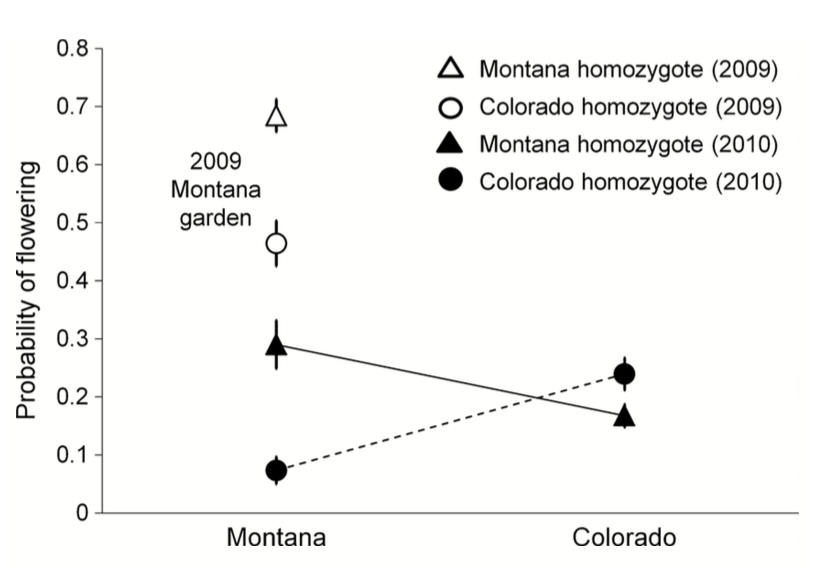
\includegraphics[width=0.7\textwidth]{boechera2.png}\\
\tiny
Adapted from \citet[Figure 3]{Anderson:2012cb}
\end{block}
\end{frame}



%%%%%%%%%%%%%%%%%%%%%%%%%%%%%%%%%%%%%%%%%%%%%%


\begin{frame}
\frametitle{Before we get started, let's set the stage for where we are}
\begin{block}{}
\centering
\includegraphics[height=0.8\textheight]{sork}\\
\tiny
Adapted from \citet[Figure 1]{Sork:2013tb}
\end{block}{}
\end{frame}

\begin{frame}
\frametitle{Evoluationary quantitative genetics}
\begin{block}{Goals}
\begin{itemize}
\item{Understand the genetics and inheritance of complex traits}
\item{Nature and strength of evolutionary forces}
\item{Natural populations}
\end{itemize}
\end{block}

\begin{block}{Natural selection}
\begin{itemize}
\item{On traits}
\item{Heritability}
\item{Variation/Variance}
\item{Additive genetic variation}
\end{itemize}
\end{block}
\tiny
\citet{Walsh:2008}
\end{frame}

\begin{frame}
\frametitle{The data we have is from multiple sources}
\begin{block}{Our data}
\begin{itemize}
\item{A sampling of individuals}
\item{A sampling of populations made up of those individuals}
\item{Some genetic data from these individuals}
\item{Some phenotypic data about the individuals}
\item{Some data about the populations (e.g., location)}
\end{itemize}

\end{block}\end{frame}

\begin{frame}
\frametitle{There are several things we'd like to do with our data}

\begin{block}{Genetic architecture}cde
\begin{itemize}
\item{Ascertain a meaningful set of genetic variants which sufficient
discriminatory power}
\item{Use this genetic variation to understand something about the 
traits of the organism we care about}
\item{In other words, given a set of traits that we observe in nature, and as
scientists we find interesting, can we attribute variation in that trait with
variation in the genome}
\end{itemize}
\end{block}
\end{frame}

\begin{frame}
\frametitle{There is some math we need}
\begin{block}{}
\begin{equation}
\label{eqn:V_P}
V_P = V_G + V_E + V_{GE}
\end{equation}

\begin{equation}
\label{eqn:V_G}
V_G = V_A + V_D + V_I
\end{equation}

\begin{equation}
\label{eqn:V_A}
V_A = 2pq\alpha^2
\end{equation}

\begin{equation}
\label{eqn:alpha}
\alpha = a + d(q-p)
\end{equation}

\begin{equation}
\label{eqn:a}
a = \frac{G_{AA}-G_{aa}}{2}
\end{equation}

\begin{equation}
\label{eqn:d}
d = G_{Aa} - \frac{G_{AA}+G_{aa}}{2}
\end{equation}

\end{block}{}
\end{frame}

\begin{frame}
\frametitle{Variance components}
\begin{block}{Equation \ref{eqn:V_P}: $V_P = V_G + V_E + V_{GE}$}
\begin{itemize}
\item{$V_P$: Phenotypic variance ($\sigma^2_P$)}
\item{$V_G$: Genetic variance}
\item{$V_E$: Environmental variance}
\item{$V_{GE}$: Genetic*environment}
\end{itemize}
\end{block}
\end{frame}

\begin{frame}
\frametitle{Genetic variance}
\begin{block}{Equation \ref{eqn:V_G}: $V_G = V_A + V_D + V_I$}
\begin{itemize}
\item{$V_G$: Total genetic variance}
\item{$V_A$: Additive genetic variance}
\item{$V_D$: Dominance genetic variance}
\item{$V_I$: Epistatic genetic variance (I = interaction)}
\end{itemize}
\end{block}
\end{frame}

\begin{frame}
\frametitle{Additive gentic variance}
\begin{block}{}
\begin{itemize}
\item{Contribution of these alleles to a phenotype are independent of 1) other
genes and 2) the environment}
\item{When multiple alleles contribute to a single phenotype (polygenic), their
presence has a linear effect on the phenotype}
\item{$V_A$ is the target of natural selection}
\end{itemize}
\end{block}{}
\end{frame}

\begin{frame}
\frametitle{Heritability}
\begin{block}{The Breeder's equation}
\begin{center}
\huge
$R = h^2S$
\end{center}
\begin{itemize}
\item[]{$R$: response to selection}
\item[]{$h^2$: narrow sense heritability ($\frac{V_A}{V_P}$)}
\item[]{$S$: selection coefficient}
\end{itemize}
\end{block}

\begin{block}{Example}
\href{http://localhost:8888/notebooks/heritability.ipynb}{heratibility.ipynb}
\end{block}
\end{frame}





\begin{frame}
\begin{block}{Popgen}
\begin{itemize}
\item{Diverse data sets (SNPs, microsatellites): DNA sequence variation,
$F_{ST}$, $Q_{ST}$}
\item{Conculsions driven by data type}
\item{Requires a reference genome}
\item{Normal challenges of next-gen data apply (quality filtering, redundancy,
coverage)}
\end{itemize}
\end{block}
\end{frame}

\begin{frame}
\frametitle{Methods to detect local adaptation}
\begin{block}{Association Mapping}
\begin{itemize}
\item{Sampling from populations}
\item{Much lower LD among loci}
\item{Needs dense sets of markers (varies with LD and genome size)}
\item{Must consider genetically differentiated populations, population
structure is important!}
\end{itemize}
\end{block}
\end{frame}

\begin{frame}
\frametitle{Association mapping in conifers}
\begin{block}{GWAS in trees}
\begin{itemize}
\item{Forest trees are important economically and environmentally}
\item{Studying them in traditional ways (i.e., QTL) is difficult: generation
time is long, phenotype not present in seedlings (e.g, wood/bark)}
\item{Complex demography, population structure, local adaptation can confound 
associations}
\item{Heritability tends to be low for traits of interest}
\item{Mapping populations may not generalize to natural populations}
\end{itemize}
\end{block}
\tiny
\citet{Uchiyama:2013ci}
\end{frame}

\begin{frame}
\frametitle{Association mapping in conifers}
\begin{block}{Conifer genomes}
\begin{itemize}
\item{Huge: \SIrange{10}{30}{GB}}
\item{Highy complex (repeats, gene content, GC-bias)}
\item{Ratio of genetic to physical distance $>$\SI{3000}{kb \per cM}}
\item{Rapid decay of LD in coding regions}
\end{itemize}
\end{block}
\tiny
\citet{Uchiyama:2013ci,Hirschhorn:2005cka}
\end{frame}

\begin{frame}
\frametitle{Association mapping in conifers}
\begin{block}{Identifying variants}
Two main methods:
\begin{itemize}
\item{Genotyping arrays}
\item{Gentoyping by sequencing (GBS)}
\item{Each have own set of biases and problems}
\end{itemize}
\end{block}
\end{frame}

\begin{frame}
\frametitle{Now that you have identified variants...}
\begin{block}{Let's revisit what you want to do}
\centering
You want to understand how the variation in your biologically important and
interesting trait is attributable to the underlying additive genetic variation 
present (i.e., heritability) in your samples (and hopefully the population).
\end{block}
\end{frame}

